\subsection{Photograph-Preserving Rank Embedding}
\label{sec:cover-method}
A separate profile, \texttt{cover\_rank\_v1}, carries the same text packet through small changes to a $256\times256$ RGB8 photograph. For each channel define $B(c)=4\lfloor c/4\rfloor$ and require $B(y)=B(x)$ for cover $x$ and carrier $y$. Both endpoints therefore reconstruct the canonical context $B+2$ without the receiver knowing $x$. An $8\times8$ row-major grid of $32\times32$ tiles supplies full parameter maps with 64 GPU forwards. The checkpoint, float32 normalization and CUDA graph settings remain unchanged.

For each selected pixel, enumerate all 64 colors in its three four-value channel cells. Their scores are
\begin{equation}
\ell(r,g,b)=\log\sum_k w_k f_{k,R}(r)f_{k,G}(g\mid r)f_{k,B}(b\mid r,g).
\end{equation}
The candidate's own preceding channels determine green and blue means. Float64 log-domain evaluation retains all 64 candidates, even if exponentiating a score would underflow. Descending scores, with lexicographic RGB ties, define zero-based ranks. Rank parity gives two 32-color bit classes. The sender chooses the nearest squared-RGB-distance candidate in the required class, with lexicographic distance ties. The receiver reads the observed rank parity. These are coarse-context embedding ranks, not the generated mode's likelihood conditioned on full-precision delivered history.

Placement derives a key with HKDF-SHA256 from the run key, salt SHA256 of row-major coarse RGB bytes, and domain-separated info binding the agreed protocol hash. The domain is \texttt{ImageCalgacus/cover\_rank\_v1/placement}, followed by a zero byte and the hash. The hash covers canonical sorted-key JSON of the model and rank rules, excluding arm and runtime paths. HMAC-SHA256 priorities use \texttt{pixel}, a zero byte and each four-byte big-endian raster index. Sorting priorities, then indices for ties, selects 2,336 distinct positions in packet-bit order, most-significant bit first. The hidden nonce is not a placement input. The paired model-free baseline labels the identical candidate cube by $(r+g+b)\bmod2$, using the same positions, sealed packet and nearest-distance rule.

The receiver receives only PNG, profile/arm and key. Cell invariance yields the same tiles, selected positions and rank map, so observed parity inverts every bit before authenticated parsing. Each channel changes by at most three. With only 2,336 selected pixels, pooled RGB MSE is at most $9(2336)/65536$, giving the conservative theoretical bound $\mathrm{PSNR}\geq53.07$ dB. Authentication protects the recovered packet, not every unused cover pixel.

\begin{figure*}[t]
\centering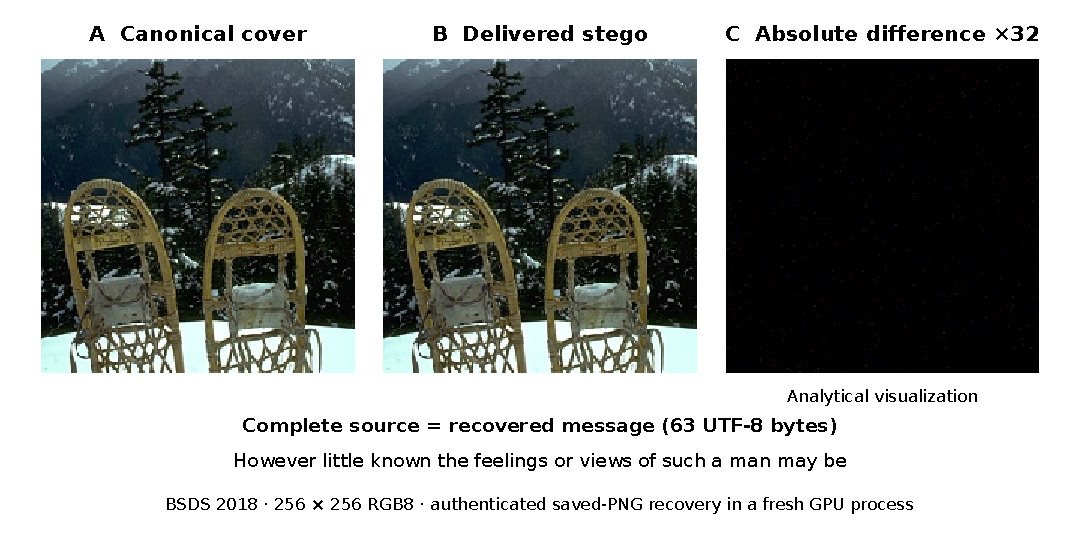
\includegraphics[width=\textwidth]{figures/cover_transport_submission.pdf}
\caption{Complete photograph transport for the same predetermined BSDS500 test case, 2018 \cite{bsds}. A is the canonical cover and B the actual delivered model-rank PNG, both $256\times256$ RGB8 at identical display scale without enhancement. C is an analytical visualization, $32|B-A|$ per RGB channel, not a carrier transformation. Black denotes no change. The shared text annotation gives the entire source and exactly recovered message. A fresh GPU receiver reconstructs the coarse context and ranks from B using only its profile and key. Authentication and independent byte equality pass.}
\label{fig:cover-example}
\end{figure*}
